\documentclass[11pt,answers]{exam}

\usepackage{etex}
\usepackage{amssymb,amsmath,multicol} %<-- InWorksheetExam1 i also have fancyhdr,

\usepackage[metapost]{mfpic}
\usepackage[pdftex]{graphicx}

\usepackage{pst-plot}
\usepackage{pgfplots}
\pgfplotsset{compat=1.9}

\usepackage{tikz}
\usepackage{tkz-2d}
\usepackage{tkz-base}
\usetikzlibrary{calc}

\usepackage[inline]{enumitem}
\usepackage{refcount}%<-- non in WorksheetExam1

%\renewcommand{\headrulewidth}{0pt}

\newcommand{\vasymptote}[2][]{
    \draw [densely dashed,#1] ({rel axis cs:0,0} -| {axis cs:#2,0}) -- ({rel axis cs:0,1} -| {axis cs:#2,0});
}

\addpoints
%\printanswers
\noprintanswers

\opengraphsfile{Q6b_Spring_15}

\begin{document}
\extrawidth{-0.3in}
\pagestyle{headandfoot}

\setlength{\hoffset}{-.25in}

\extraheadheight{-.4in}
\runningheadrule
\firstpageheader{\bfseries {MATH1-UC 1171}}{ \bfseries {QUIZ 6 }}{\bfseries {4/7/2015}} 



\firstpagefooter{} %%&&CHANGED
                {}
                {Points earned: \hbox to 0.5in{\hrulefill}
                 out of  \pointsonpage{\thepage} points}
                 
						

\vspace*{0.7cm}
\hbox to \textwidth { \scshape {Name:} \enspace\hrulefill}
\vspace{0.2in}




\pointpoints{point}{points}

\begin{questions}


\addpoints

\question Let $\displaystyle g(x)=2^{x-1}+1$.
\begin{parts}


\part[2] List the function transformations of $ \displaystyle f(x)=2^x$ that result in $g(x)$.
\fillwithdottedlines{1in}

\part[3] Graph $g(x)$. [Include units, label the $y$-coordinate of the $y$ intercept and draw the horizontal asymptote as a dashed line.]

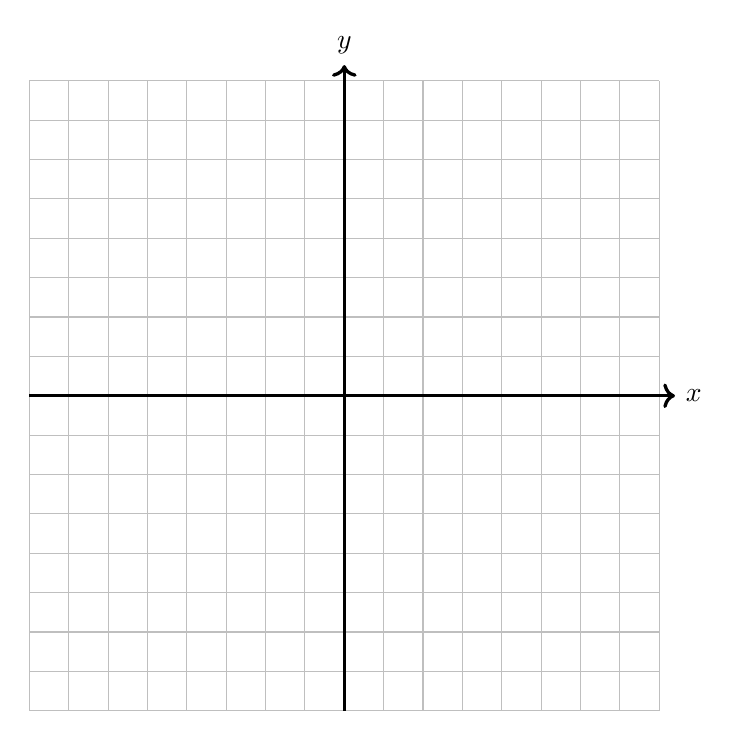
\begin{tikzpicture}

    \draw[gray!50, thin, step=0.5] (-4,-4) grid (4,4);
    \draw[very thick,->] (-4,0) -- (4.2,0) node[right] {$x$};
    \draw[very thick,->] (0,-4) -- (0,4.2) node[above] {$y$};

\end{tikzpicture}

\part[2] Write the range of $g(x)$ in interval form. \hbox to 0.9in{\dotfill}

\part[1] Write the equation of the horizontal asymptote of $g(x)$. \hbox to 0.9in{\dotfill}
\end{parts}
\question[2] If \$100,000 is invested at an interest rate of 0.5\% per year, compounded quarterly, write a formula to find the value of the investment after 1 year.

\fillwithdottedlines{1in}

%%%%%%%%%%%%%%%%%%%%%%%%%%



\end{questions}

\end{document}                 